\documentclass[11pt]{article}

\usepackage{amsmath, amssymb, amsthm, graphicx, xcolor}

\newcommand{\red}[1]{\textcolor{red}{#1}}

\title{Tur\'an Formulas}
\author{S. Coniglio}
\date{}

\begin{document}

\maketitle


\section{Tur\'an's formula, 1941}

Let $n \ge k \ge 3$. Tur\'an's graph $D(n,k)$ (original notation) is a balanced $(k-1)$-partite graph on $n$ vertices. A depiction of $D(7,4)$ taken from Tur\'an's paper is the following one:

\begin{center}
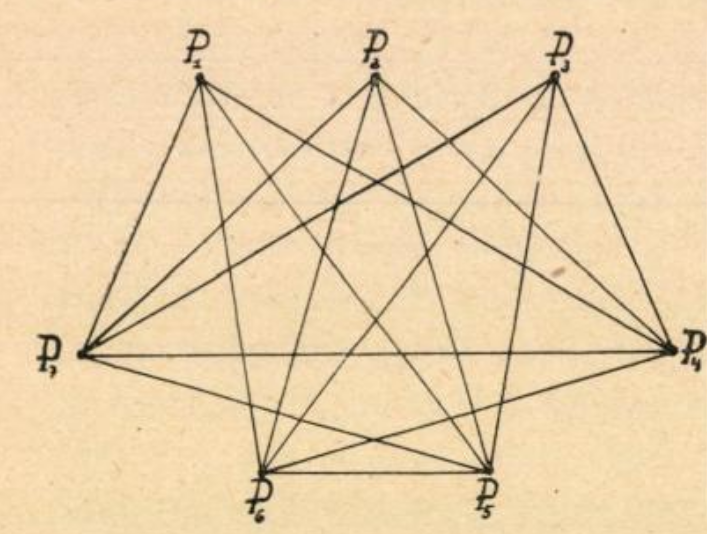
\includegraphics[width=0.7\textwidth]{images/20260215184633.png}
\end{center}


Let $d_k(n)$ (original notation---maybe for {\em density}?) be the size of the largest graph on $n$ nodes that is $K_k$-free. Tur\'an proves that such a graph is $D(n,k)$, that it is \red{unique} (check), and that its size is
\[
d_k(n) = \frac{k-2}{2(k-1)}\,(n^2 - r^2) + \binom{r}{2},
\]
where
% $r$ is defined by
% \[
% n \equiv r \pmod{k-1}, \qquad 0 \le r < k-1.
% \]
\[
n = (k-1) t + r, \qquad 0 \le r \le k-2.
\]

\section{Wolfram formula (just a bound)}

\begin{center}
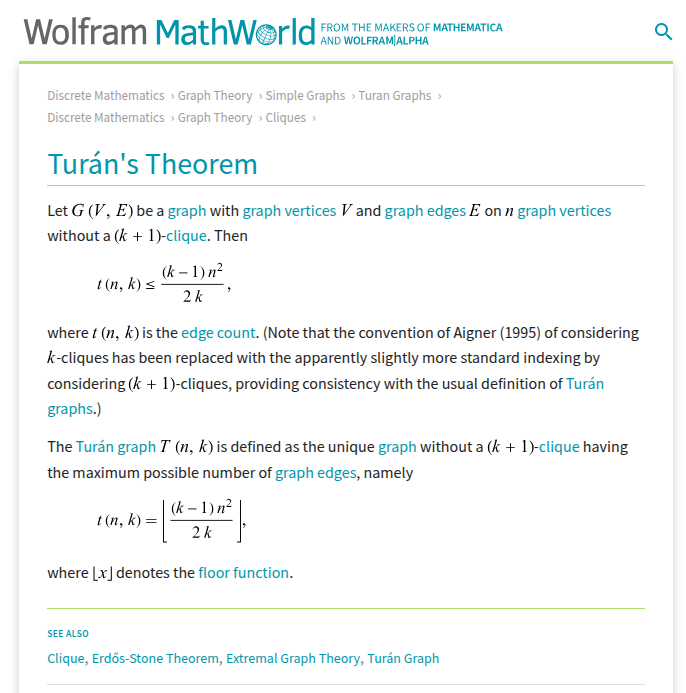
\includegraphics[width=0.7\textwidth]{images/20260217223229.png}
\end{center}

Modified version for the $K_k$-free case (and not $K_{k_1}$-free as in the webpage):
\[
d_k(n) \le \left\lfloor \frac{(k-2)n^2}{2(k-1)}  \right\rfloor.
\]


\section{Counting formula, origin unknown (folklore?)}


The balanced $(k-1)$-partite Tur\'an graph has:
\begin{itemize}
    \item $r$ parts of size $t+1$,
    \item $k-1-r$ parts of size $t$.
\end{itemize}

It is immediately obvious that $d_k(n)$ is equal to the total possible number of edges minus the intra-part edges:

\[
d_k(n)
=
\binom{n}{2}
-
r \binom{t+1}{2}
-
(k-1-r)\binom{t}{2}.
\]


\subsection{Derivation}


\subsubsection*{Step 1: Expand the binomial coefficients}

\[
d_k(n)
=
\frac{n(n-1)}{2}
-
r \frac{t(t+1)}{2}
-
(k-1-r)\frac{t(t-1)}{2}.
\]

Factor out $\frac{t}{2}$ from the last two terms:

\[
d_k(n)
=
\frac{n(n-1)}{2}
-
\frac{t}{2}
\left[
r(t+1)
+
(k-1-r)(t-1)
\right].
\]

\subsubsection*{Step 2: Simplify the bracket}

\[
r(t+1)
+
(k-1-r)(t-1)
=
rt + r
+
(k-1)t - (k-1) - rt + r
=
(k-1)t + 2r - (k-1).
\]

Thus,

\[
d_k(n)
=
\frac{n(n-1)}{2}
-
\frac{t}{2}
\left(
(k-1)t + 2r - (k-1)
\right).
\]

\subsubsection*{Step 3: Use $n=(k-1) t + r$}

Since $(k-1)t = n - r$, we have

\[
(k-1)t + 2r - (k-1)
=
(n-r) + 2r - (k-1)
=
n + r - (k-1).
\]

Therefore,

\[
d_k(n)
=
\frac{n(n-1)}{2}
-
\frac{t}{2}
(n+r-(k-1)).
\]

Substitute $t = \frac{n-r}{k-1}$:

\[
d_k(n)
=
\frac{n(n-1)}{2}
-
\frac{1}{2}
\cdot
\frac{n-r}{k-1}
(n+r-(k-1)).
\]

\subsubsection*{Step 4: Put over common denominator $2(k-1)$}

\[
d_k(n)
=
\frac{
(k-1)n(n-1)
-
(n-r)(n+r-(k-1))
}{2(k-1)}.
\]

Expand:

\[
(k-1)(n^2-n)
-
\big(
n^2 + nr - n(k-1) - nr - r^2 + r(k-1)
\big)
=
(k-1)n^2 - (k-1)n - n^2 + n(k-1) + r^2 - r(k-1).
\]

Simplify:

\[
=
(k-2)n^2 + r^2 - r(k-1).
\]

Hence,

\[
d_k(n)
=
\frac{(k-2)n^2 + r^2 - r(k-1)}{2(k-1)}
=
\frac{k-2}{2(k-1)}n^2
+
\frac{r(r-(k-1))}{2(k-1)}.
\]

Finally,

\[
\boxed{
d_k(n)
=
\frac{k-2}{2(k-1)}n^2
-
\frac{r(k-1-r)}{2(k-1)}
=
\frac{k-2}{2(k-1)}\,(n^2-r^2) + \binom{r}{2}.
}
\]

\end{document}
